\documentclass[11pt, letterpaper]{article}
\usepackage[margin=2cm]{geometry}
\usepackage{fourier}
\usepackage[T1]{fontenc}
\usepackage[utf8]{inputenc}
\usepackage{amsmath}
\usepackage{bookmark}
\usepackage{hyperref}
\usepackage{booktabs}
\usepackage{multicol, caption}
\newenvironment{Figure}
  {\par\medskip\noindent\minipage{\linewidth}}
  {\endminipage\par\medskip}
\usepackage{cite}
\usepackage{graphicx}
\usepackage{wrapfig}
\providecommand{\tightlist}{%
  \setlength{\itemsep}{0pt}\setlength{\parskip}{0pt}
}
\setlength{\columnsep}{1cm}
\setcounter{secnumdepth}{-\maxdimen}
\title{Fighting Fakes Fairly}

\author{
  Alex Kyllo
  \and
  John Wyman
  \and
  Will Thomas
}

\begin{document}

\maketitle

\begin{abstract}
  In this study we investigate whether it is still feasible to
  automatically discern AI-generated human face images from genuine
  photographic ones, by training a convolutional neural network on a
  labeled dataset of 70,000 real and 70,000 fake face images. We use
  the fake face classification problem to further explore the topic of
  model fairness, by evaluating the model's performance across age,
  gender and race groups on a demographically labeled face dataset. To
  achieve this, we propose a method of utilizing an autoencoder
  network to translate demographically labeled real face images into
  an approximation of their latent space code representations and then
  reconstruct them back into images, creating a dataset of matching
  fake face images with the same demographic labels. This allows us to
  assess whether our fake face detection model works equally well for
  human faces of different age, gender and race groups, or whether it
  even generalizes to a dataset that is demographically diverse and
  balanced. Our source code is published at
  \href{https://github.com/alexkyllo/fake-faces/}{github.com/alexkyllo/fake-faces}.
\end{abstract}

\begin{multicols}{2}
  \section{Introduction}

  Generative Adversarial Networks (GANs) have created the ability to
  encode photographic images into a latent space representation and
  automatically generate many images that can appear to be genuine
  photographs, to the human eye. NVIDIA's
  \emph{StyleGAN}\cite{stylegan} model, trained on a dataset of human
  face images, is capable of generating extremely photo-realistic
  images of people who do not exist. \emph{StyleGAN} is an example of
  a generative adversarial network (GAN), a type of network that
  consists of two models, a \emph{generator}, which learns a data
  distribution from a training set and draws from it, and a
  \emph{discriminator}, which learns to estimate the probability that
  a sample came from the training data or from the generator
  \cite{goodfellow2014generative}.

  The application of GANs to generating realistic human faces has
  garnered much media attention in recent years. The well-known
  website \href{https://thispersondoesnotexist.com/}{This Person Does
    Not Exist} serves random, high-resolution fake face images drawn
  from \emph{StyleGAN}. Many models have been created for exploring
  the latent space of \emph{StyleGAN} to discover vectors that
  correspond to semantic directions in which the latent codes can be
  perturbed in order to make semantic edits to human face photos, such
  as making the face look older vs. younger, more masculine vs. more
  feminine \cite{shen2020interpreting}, or thinner vs. heavier
  \cite{pinnimty2020transforming}. The popular mobile application
  FaceApp utilizes this method to allow users to transform images of
  themselves in this manner and share them on social media for
  humor. Two different people's face images can also be blended
  together by encoding both images and interpolating some point
  between them in the latent space, which can be used for applications
  like visualizing what a couple's children might look like, a concept
  that has been implemented in the project
  \href{https://medium.com/swlh/familygan-generating-a-childs-face-using-his-parents-394d8face6a4}{FamilyGAN}.

  It is also easy to imagine nefarious applications of fake face
  generation, some of which have already been realized, such as
  swapping faces of celebrities onto pornographic actors or falsifying
  speeches by political leaders \cite{nguyen2020deep}. Because such
  applications of this technology can unfairly damage people's
  reputations and erode trust in society, there is a public interest
  in retaining the ability to effectively discern real human face
  images and video from fake ones and detect "deep fake" tampering,
  which requires training more deep learning models to distinguish
  them.

  A problem with the available open datasets of human faces used in
  training deep learning models, is bias in the demographic
  composition of the pictured individuals. The machine learning
  community has recently been struggling with the issue of model
  fairness--it is important that models perform equitably for users
  and data subjects of different backgrounds, and also very difficult
  to enumerate and quantify the sources of bias in training data that
  can contribute to biased model performance.

  The \emph{FairFace}\cite{karkkainen2019fairface} study introduced a new
  dataset of human face images collected from public datasets with
  manually verified, crowdsourced age, gender and race labels. The
  \emph{FairFace} paper demonstrates that because existing public datasets of
  human faces contain a majority of white faces, models trained on
  them fail to generalize well to datasets where more non-white faces
  are present. We suspected that this might also be the case for the
  \emph{140k Real and Fake Faces} dataset that we utilized for model
  training, and sought to test this by evaluating it on a
  demographically labeled dataset.

  While the \emph{FairFace} dataset provides real human face images
  that can be used to assess disparities in a fake face detector's
  true negative and false positive rates, a second, similarly labeled
  dataset of fake face images is needed to compute true positive and
  false negative rates for specific age, gender and race groups. To
  address this gap, we investigated methods for ``falsifying'' a real
  face image by autoencoding it via the \emph{StyleGAN} latent
  space. A research team at Tel Aviv University recently developed a
  novel encoder network\cite{richardson2020encoding} called
  \emph{pixel2style2pixel}, that is capable of approximately
  reconstructing \emph{StyleGAN}'s latent code representation of a
  face image and then decoding it back into an image. This yields a
  fake face output image that very closely resembles the real face
  input image, implying that the original demographic labels would
  remain valid, and giving us a dataset of matching real and fake
  faces for scoring our models and calculating classifier fairness
  metrics.

  \section{Methods}

  \subsection{Training Dataset}

  Our primary dataset for training was the
  \href{https://www.kaggle.com/xhlulu/140k-real-and-fake-faces}{\emph{140k
    Real and Fake Faces} dataset from user \emph{xhlulu} on
    Kaggle}. The dataset consists of all 70,000 real faces from the
  Flickr dataset collected by NVIDIA, plus 70,000 fake face images
  generated by \emph{StyleGAN}. All images were provided in 256x256x3
  resolution. The dataset was pre-split into a test set and validation
  set of 10,000 real and 10,000 fake faces each, with the remaining
  100,000 images as the training set.

  Our secondary dataset, used for the fairness assessment, was the
  \href{https://github.com/joojs/fairface}{\emph{FairFace} dataset}
  \cite{karkkainen2019fairface}, which consists of 86,744 training
  images and 10,954 test images, labeled with the following
  crowdsourced demographic labels (Tables \ref{genders}, \ref{races},
  \ref{ages}).

  \begin{Figure}
    \captionof{table}{Genders labeled in \emph{FairFace} dataset}
    \label{genders}
  \begin{tabular}{lr}
    \toprule
        gender &  count  \\
        \midrule
        Female &  45920 \\
        Male   &  51778 \\
        \bottomrule
  \end{tabular}
  \end{Figure}

  \begin{Figure}
    \captionof{table}{Races labeled in \emph{FairFace} dataset}
    \label{races}
  \begin{tabular}{lr}
    \toprule
        race            &  count \\
        \midrule
        Black           &  13789 \\
        East Asian      &  13837 \\
        Indian          &  13835 \\
        Latino\_Hispanic &  14990 \\
        Middle Eastern  &  10425 \\
        Southeast Asian &  12210 \\
        White           &  18612 \\
        \bottomrule
  \end{tabular}
  \end{Figure}

  \begin{Figure}
    \captionof{table}{Ages labeled in \emph{FairFace} dataset}
    \label{ages}
  \begin{tabular}{lr}
    \toprule
        age          &  count \\
        \midrule
        0-2          &   1991 \\
        3-9          &  11764 \\
        10-19        &  10284 \\
        20-29        &  28898 \\
        30-39        &  21580 \\
        40-49        &  12097 \\
        50-59        &   7024 \\
        60-69        &   3100 \\
        more than 70 &    960 \\
        \bottomrule
  \end{tabular}
  \end{Figure}

  Unfortunately the gender variable is limited to a binary Male/Female
  as \emph{FairFace} does not include labels for nonbinary
  individuals, and the race label is also limited to just seven race
  groups, some of which are arguably ethnicities rather than races.
  The \emph{FairFace} paper\cite{karkkainen2019fairface} discusses
  these limitations in depth, providing explanations of the practical
  considerations and difficulties in labeling more granular identities
  from open face image datasets.

  \subsection{Data Preprocessing and Augmentation}

  We tested several methods for preprocessing and augmenting the image data
  before feeding it into the CNN model.

  \begin{itemize}
    \tightlist
  \item 3-color (RGB) images vs. grayscale
  \item Pre-cropping and centering faces using pre-trained face
    detection models
  \item Random horizontal flips, rotations, and shears
  \end{itemize}

  Before training our CNN models we pre-cropped the images to center
  and align the faces with eyes, nose and mouth level. We utilized two
  different pre-trained face detection models. The first model we used
  was the Multi-Task Cascaded Convolutional Neural Network (MTCNN)
  \cite{Zhang_2016}. Later, we switched to utilizing the Dlib package
  implementation of the Shape Predictor 68 Face Landmarks model
  \cite{SAGONAS20163} because the \emph{pixel2style2pixel} model was
  trained on face images that were aligned with this model, so it
  expects the input to conform to this particular alignment.

  \subsection{Model Training}

  To solve the binary classification task of distinguishing between
  real and fake human face images, we trained several variations of
  deep Convolutional Neural Networks (CNN), varying the number of
  convolution layers as well as several model hyperparameters and
  image preprocessing steps. We utilized the TensorFlow Keras API and
  trained the model on a single consumer-grade
  GeForce\texttrademark\ RTX 20 series GPU, demonstrating that this
  problem is manageable even without access to institutional
  high-performance computing resources.

  Our intial baseline model was a CNN with three convolution layers
  using a 3x3 element kernel. We trained it on grayscale images from
  the \emph{140k Real and Fake Faces} dataset, cropped using MTCNN, with no
  image augmentations applied. The baseline model's learning curves
  over training 20 epochs are pictured in Figure
  \ref{learning-curve-baseline}.

  \begin{Figure}
    \centering
    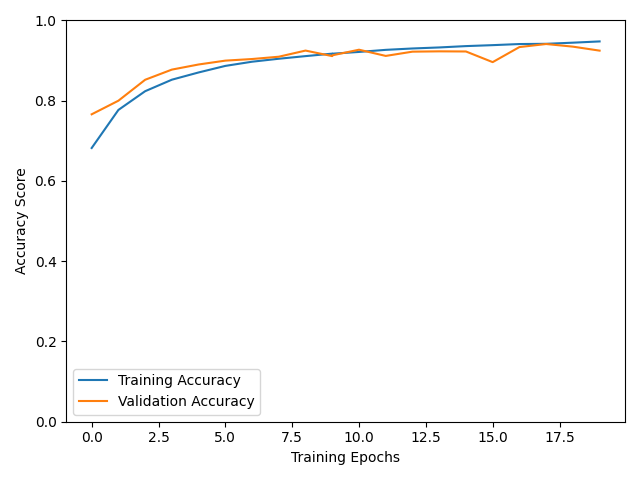
\includegraphics[width=1.0\textwidth]{figures/learning-curve-baseline-cropped-grayscale-noaug.png}
    \captionof{figure}{Learning curve for baseline model trained on fake faces grayscale images}
    \label{learning-curve-baseline}
  \end{Figure}

  Figure \ref{learning-curve-vgg10-combined} and Figure
  \ref{learning-curve-vgg10-rgb-combined} depict the learning curves
  for our best VGG-10 model, trained on the combined dataset in
  grayscale and RGB, respectively. Using RGB color images did not
  appear to offer a significant benefit, as both models were able to
  exceed 98\% validation accuracy within fewer than 20 training
  epochs.

  \begin{Figure}
    \centering
    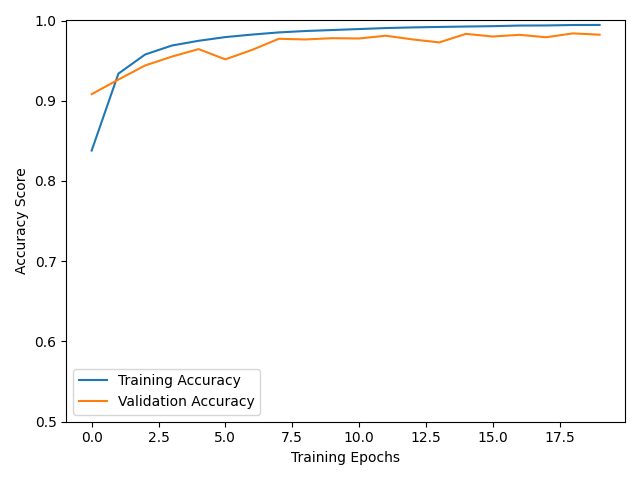
\includegraphics[width=1.0\textwidth]{figures/learning-curve-vgg10-dlib-hflip-combined-125-0001.png}
    \captionof{figure}{Learning curve for VGG-10 model trained on combined grayscale images}
    \label{learning-curve-vgg10-combined}
  \end{Figure}

  \begin{Figure}
    \centering
    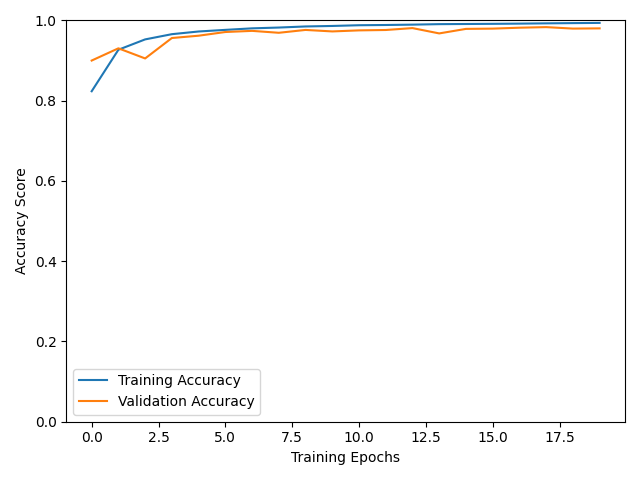
\includegraphics[width=1.0\textwidth]{figures/learning-curve-vgg10-dlib-hflip-rgb-combined-125-0001.png}
    \captionof{figure}{Learning curve for VGG-10 model trained on combined RGB images}
    \label{learning-curve-vgg10-rgb-combined}
  \end{Figure}

  We experimented with several other, more complex model
  architectures, including a deeper VGG-16 model, a ResNet-50 model,
  and a DenseNet-121 model, but found that those models tended to
  overfit the training set, whereas the baseline 3-layer model
  underfit compared to the VGG-10 model.

  \subsection{Model Serving}

  To make our model available on the internet, we developed a web
  application with a simple UI form that allows the user to provide a
  URL or file upload of a human face image.  The application calls the
  Keras model to retrieve a prediction and displays a message
  indicating whether it is likely a real face or a fake (Figure
  \ref{fake-faces-web}). We built it using a small amount of Vue.js
  and Python code and deployed it to Azure Functions as a
  ``serverless'' application, eliminating the need to manage any server
  infrastructure to operate the web site.

  \begin{Figure}
    \centering
    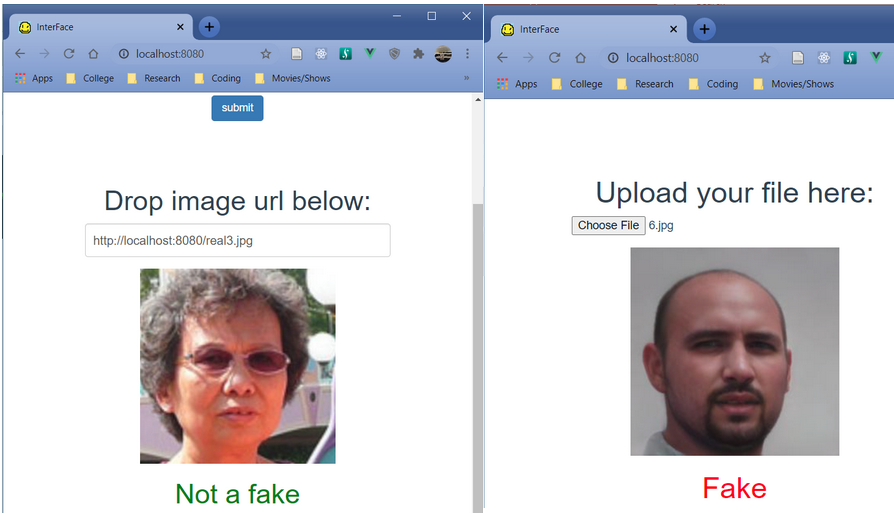
\includegraphics[width=1.0\textwidth]{figures/fake-faces-web.png}
    \captionof{figure}{Screenshot of fake face inference web application}
    \label{fake-faces-web}
  \end{Figure}

  \subsection{Model Evaluation}

  Our primary metric for performance assessment during training and
  model selection was validation set accuracy, because the balanced
  classes of the input dataset made accuracy straightforward to
  interpret. For final model performance on out-of-sample test data,
  we report performance using F1 score, precision score and recall
  score in addition to accuracy score, to communicate how well the
  model performed across a variety of standard binary classifier
  metrics.

  For fairness metrics, we selected two standard binary classifier
  metrics to evaluate our classifier on: disparate impact ratio, given
  by the ratio of the rate of positive predictions for the
  unprivileged class to that of the privileged class
  \cite{fairMLHealth}, given by:

  $$\frac{P(\hat{y}|unprivileged)}{P(\hat{y}|privileged)}$$

  and average odds difference, given by:

  $$\frac{(FPR_{unpriv} - FPR_{priv}) + (TPR_{unpriv} - TPR_{priv})}{2}$$

  for the following binary group definitions taken from the \emph{FairFace}
  labels:

  \begin{enumerate}
    \tightlist
  \item Gender = ``Male'' vs Gender = ``Female''
  \item Race = ``White'' vs all other races
  \item Race = ``Black'' vs all other races
  \item Age = ``0-2'' vs all other ages
  \item Age = ``3-9'' vs all other ages
  \item Age = ``more than 70'' vs all other ages
  \end{enumerate}

  We examine the model fairness for children and senior citizens as a recent
  study \cite{9156262} found that the popular face recognition model Face++
  disproportionately fails to recognize children's faces in images collected
  from social media.

  \section{Results}

  We determined that the fake face classification task is still
  achievable with a relatively simple CNN model, but that model also
  failed to generalize to the unseen \emph{FairFace} dataset, so we
  refined the model on additional training examples from
  \emph{FairFace} to correct this. Below we detail our findings at
  each stage of the process.

  \subsection{Preprocessing Results}

  We utilized two pre-trained face recognition models to locate the human face
  in the image, align it so that the eyes, nose and mouth are level and
  centered, and crop to a margin around the face. Because these preprocessing
  models are themselves probabilistic machine learning models, they sometimes
  fail to recognize a human face at all (false negative) or incorrectly
  recognize some other object as a human face (false positive). We examined the
  images for which face detection failed.

  The Dlib frontal face detector method mistook several objects including a logo
  and a necklace for human faces (Figure \ref{falsepos}), while the MTCNN face
  detector method failed to identify several faces with brightly colored hair or
  wigs and heavy makeup as faces (Figure \ref{falseneg})

  \begin{Figure}
    \centering
    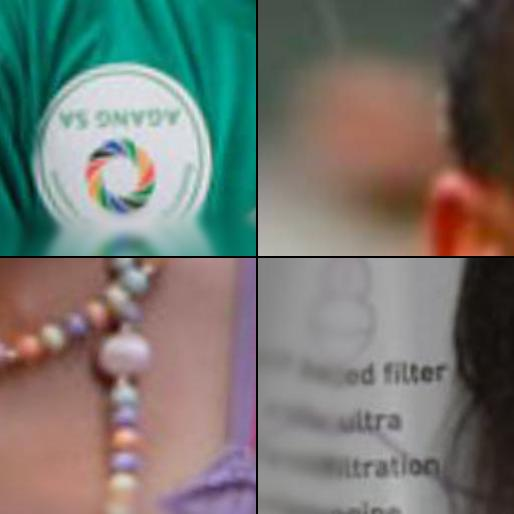
\includegraphics[width=0.7\textwidth]{figures/false-positives.jpg}
    \captionof{figure}{Sample of false positives cropped by Dlib.}
    \label{falsepos}
  \end{Figure}

  \begin{Figure}
    \centering
    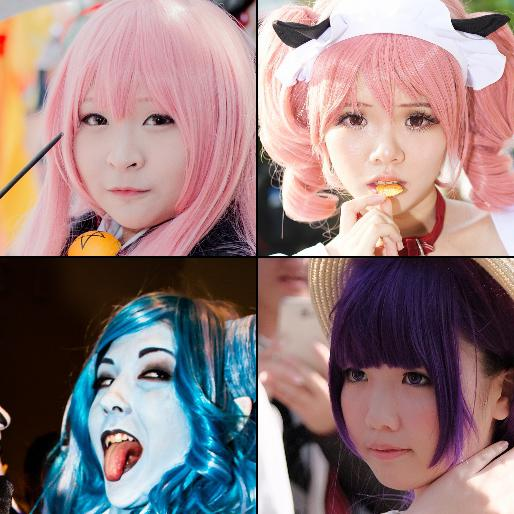
\includegraphics[width=0.7\textwidth]{figures/false-negatives.jpg}
    \captionof{figure}{Sample of false negatives that MTCNN failed to crop.}
    \label{falseneg}
  \end{Figure}

  By applying the \emph{pixel2style2pixel} encoding algorithm to the
  \emph{FairFace} images, we were able to successfully obtain a
  dataset of 79,484 matching pairs of real and fake faces with
  verified age, race, and gender labels.

  \begin{Figure}
    \centering
    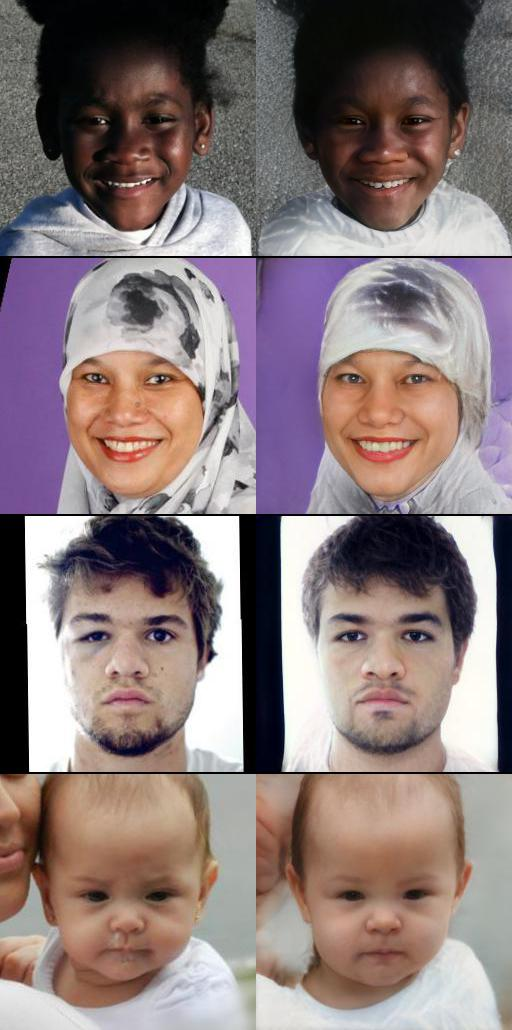
\includegraphics[width=0.7\textwidth]{figures/fair2fake.jpg}
    \captionof{figure}{Selected \emph{FairFace} images before/after
      encoding by pixel2style2pixel}
    \label{fair2fake}
  \end{Figure}

  \subsection{Model Performance Results}

  The baseline model achieved the following performance on the Fake Faces test
  set, after 18 training epochs (Table \ref{baseline-metrics}):

  \begin{Figure}
    \captionof{table}{Baseline model performance}
    \label{baseline-metrics}
    \begin{tabular}{rrrr}
    \toprule
     Accuracy &        F1 &  Precision &    Recall \\
    \midrule
     0.942197 &  0.941569 &   0.951865 &  0.931493 \\
    \bottomrule
    \end{tabular}
  \end{Figure}

  Our best model in hyperparameter tuning was a variant of the VGG architecture
  \cite{simonyan2015deep} with 10 total layers (8 convolution layers and 2 fully
  connected layers). This model's performance is given by
  (Figure \ref{vgg10-fakeface-metrics}).

  \begin{Figure}
    \centering
    \captionof{table}{Best (VGG10) Model performance on Fake Faces test set}
    \label{vgg10-fakeface-metrics}
    \begin{tabular}{rrrr}
    \toprule
     Accuracy &        F1 &  Precision &    Recall \\
    \midrule
     0.968298 &  0.967689 &   0.986595 &  0.949495 \\
    \bottomrule
    \end{tabular}
  \end{Figure}


  \subsection{Fairness Assessment Results}

  Our best model trained on the \emph{140k Real and Fake Faces}
  dataset failed to generalize to the \emph{FairFace} dataset, marking
  nearly all of the \emph{FairFace} observations as fake faces,
  resulting in high recall but very low precision and accuracy scores
  (Figure \ref{vgg10-transfer-fail}).

  \begin{Figure}
    \centering \captionof{table}{VGG10 model performance metrics on
      \emph{FairFace} after training on Fake Faces}
    \label{vgg10-transfer-fail}
    \begin{tabular}{rrrr}
    \toprule
    Accuracy &        F1 &  Precision &  Recall \\
    \midrule
      0.54305 &  0.676667 &    0.52357 &  0.9563 \\
    \bottomrule
    \end{tabular}
  \end{Figure}

  We originally intended to perform a fairness assessment on both our baseline
  model and our best model trained on the fake faces dataset, but because
  these models completely failed to generalize to the \emph{FairFace} data,
  we decided not to even assess their demographic fairness metrics. Rather, we
  retrained our best model on a combined dataset consisting of the entire
  training sets from both the \emph{140k Real and Fake Faces} and the \emph{FairFace} datasets.

  The resulting model performed very well on the combined dataset (Figure
  \ref{vgg10-combined-metrics}), and even performed better on the 70 real and
  fake faces dataset than the model version that was only trained on that
  dataset (Figure \ref{vgg10-combined-fakefaces-metrics}), suggesting that the
  additional training examples from \emph{FairFace} led to a general improvement.

  \begin{Figure}
    \centering
    \captionof{table}{Model performance metrics on \emph{FairFace} + Fake Faces combined dataset}
    \label{vgg10-combined-metrics}
    \begin{tabular}{rrrr}
    \toprule
    Accuracy &        F1 &  Precision &    Recall \\
    \midrule
    0.984457 &  0.984411 &   0.986268 &  0.982561 \\
    \bottomrule
    \end{tabular}
  \end{Figure}

  \begin{Figure}
    \centering
    \captionof{table}{Performance on Fake Faces test set for model trained on combined dataset}
    \label{vgg10-combined-fakefaces-metrics}
    \begin{tabular}{rrrr}
    \toprule
     Accuracy &        F1 &  Precision &    Recall \\
    \midrule
     0.971232 &  0.971092 &    0.97374 &  0.968458 \\
    \bottomrule
    \end{tabular}
    \end{Figure}

  Our best model, using the VGG10 architecture and trained on the combined
  dataset, achieved excellent performance by the fairness metrics, disparate
  impact ratio (where 1.0 is perfectly fair) and average odds difference
  (where 0.0 is perfectly fair).

    \begin{Figure}
      \centering
      \captionof{table}{Model Fairness metrics}
      \label{fairnessmetrics}
      \begin{tabular}{lrr}
      \toprule
      {} &  Disparate Impact &  Avg Odds Diff \\
      \midrule
      Male       &                0.993955 &                -0.000031 \\
      White      &                1.027800 &                -0.001012 \\
      Non-Black  &                1.004817 &                 0.000983 \\
      Non-Child  &                1.011344 &                 0.000167 \\
      Non-Senior &                1.003951 &                 0.001968 \\
      \bottomrule
      \end{tabular}
      \end{Figure}

  \section{Discussion}
  Our initial goal of detecting fake faces was successful on the
  original dataset, with 96.8\% test accuracy, but testing on the
  additional \emph{FairFace} data revealed its poor generalization
  capability, with test accuracy plummeting to 54.3\%. Some possible
  reasons for this generalization failure include:

  \begin{enumerate}
    \tightlist
  \item Demographic selection bias in the original training set,
    causing the model to perform poorly on a more diverse test set.
  \item Some specific pattern in the original training set unrelated to
    the real vs. fake task, causing overfitting specific to the
    \emph{140k Real and Fake Faces} dataset.
  \item Different characteristics of fake face images produced by
    \emph{pixel2style2pixel} vs. the original \emph{StyleGAN} network.
  \item Insufficient training examples in the original dataset to
    generalize to other datasets beyond it.
  \end{enumerate}

  We dealt with this issue successfully by introducing training
  examples from the \emph{FairFace} training set and retraining our
  model, a process that yielded a better and more general model
  overall, which also performs fairly across labeled gender, race and
  age groups.  We believe this demonstrates the utility of planning
  for model fairness up front, and incorporating labeled, balanced
  datasets such as \emph{FairFace}, to train models that are
  demonstrably better and more equitable.

  \subsection{Future Work}
  Overall, we are quite happy with the way our model performs, but
  there are several adjustments we want to make that could further
  increase accuracy. We do not believe that there were any fundamental
  flaws in our methods, just limitations in time, resources, and
  data. Given more time to develop and tune our model, we believe we
  could further increase its performance at the classification task
  without sacrificing fairness.

  Another potential technique to explore is an online learning model that
  collects user uploaded images and incrementally fine-tunes itself on these
  additional training examples--although this would require trusted input
  because a malicious user could upload intentially mislabeled examples.

  Furthermore, given additional time we would like to implement
  Grad-CAM\cite{Selvaraju_2019} pixel activation heatmaps for our
  model, to gain an understanding of which visual features the model
  is learning from the fake face images, and deliver a more
  explainable model.

  In 2020, NVIDIA released \emph{StyleGAN2}\cite{karras2020analyzing},
  which produces higher-quality fake faces in higher image resolution.
  These images are ostensibly harder to detect, so further work would
  be needed to fine-tune the model to learn training examples from
  this new adversary.

  In the future, we would love to incorporate these changes and apply
  more compute power to the problem. Using ample amounts of training
  data and more computer vision techniques we believe that there is
  still room to improve on our model, which indeed seems necessary to
  keep up in the digital ``arms race'' started by fake face GAN
  technology.

\end{multicols}

\bibliography{report}
\bibliographystyle{unsrt}
\end{document}
